\documentclass[12pt]{beamer}

\mode<presentation> {
	
	
	%\usetheme{Madrid}
	%\usepackage{times}
	\renewcommand{\familydefault}{\rmdefault}
	\usetheme{Darmstadt}
    \usecolortheme{crane}
	\usepackage[latin1]{inputenc}
	\usefonttheme{professionalfonts}
	\usepackage{times}
    \usepackage{color}
	\usepackage{tikz}
	\usepackage{amsmath}
	\usepackage{verbatim}
	\usepackage{enumerate}
	\usepackage{setspace}
	\usetikzlibrary{arrows,shapes}
	\usepackage{amsmath}
	\usepackage{eurosym}
	\usepackage{framed}
	\usepackage{extarrows}
    \usepackage{setspace}

}

\usepackage{graphicx}
\usepackage{booktabs}
\usepackage{url}
\setbeamercolor{footcolor}{fg=white,bg=blue!55} % ��������ͱ�����ɫ

\setbeamertemplate{footline}{%

  \leavevmode%

  \hbox{%

    \begin{beamercolorbox}[wd=.126\paperwidth,ht=2.25ex,dp=1ex,right]{footcolor}%

       \insertframenumber{} / \inserttotalframenumber\hspace*{5ex}

    \end{beamercolorbox}}%

  \vskip0pt%

}



%----------------------------------------------------------------------------------------
%	TITLE PAGE
%----------------------------------------------------------------------------------------


\title{\emph{Pricing an Asian Option by Applying the Random Numbers Generated from the Halton Sequence} }

\author[Prof.Wolfgang. H\"{a}rdle,]{\textbf{Instructor: Prof. Wolfgang. K. H\"{a}rdle}} % Your name
\institute[]{
	\textsl{\\
                         15420151152767  \quad\quad Chai Qingqing \quad\quad\quad\quad\quad  No.05              \\
                         15620151152820  \quad\quad Jin Jianfei   \hfill No.07       \\
                         15620151152828  \quad\quad Ma Shiyun     \hfill No.45              \\
                         15420151152766  \quad\quad Xu Yunkun     \hfill No.49}
}

\date[July 7$^{th}, 2016$]{} % Date, can be changed to a custom date

\begin{document}
\setlength{\baselineskip}{1.2\baselineskip}
\setbeamertemplate{footline}[frame number]

\begin{frame}
	\titlepage
\end{frame}


\begin{frame}
	\frametitle{Outline}
	\tableofcontents
\end{frame}
%----------------------------------------------------------------------------------------
\section{MONTE-CARLO METHODS}
\begin{frame}
	\frametitle{MONTE-CARLO METHODS}
\begin{spacing}{1.5}
\begin{itemize}
  \item \textsf{Monte Carlo Methods are a broad class of computational algorithms that rely on repeated {\color{red} random sampling} to obtain numerical results.}
  \item \textsf{The modern version of the Markov Chain Monte Carlo method was invented in the late 1940s by \href{https://en.wikipedia.org/wiki/Stanislaw_Ulam}{{\color{purple} Stanislaw Ulam}}}
\includegraphics[width=15pt,height=15pt]{link23.jpg} .
\end{itemize}
\end{spacing}
\end{frame}
%----------------------------------------------------------------------------------------
\begin{frame}
\frametitle{MONTE-CARLO METHODS}
\begin{itemize}
  \item \textsf{Their \textbf{\large essential idea}  is to use {\color{red} randomness} to solve problems that might be deterministic in principle. Monte Carlo methods can be used to solve any problem having a probabilistic interpretation.
  \item By {\color{red} the Law of Large Numbers (LLN)}, integrals described by the expected value of some random variable can be approximated by taking the empirical mean of independent samples of the variable.}
\end{itemize}
\end{frame}
%----------------------------------------------------------------------------------------
\begin{frame}
\frametitle{MONTE-CARLO METHODS FOR OPTION PRICING}
\textsf{A {\color{red}three-step} approach to price an option by Monte Carlo method is as follows:}\\
\begin{itemize}
  \item \textsf{Generate a large number of possible (but random) price paths for the underlying (or underlyings) via simulation.
  \item	Calculate the associated exercise value (i.e. "payoff") of the option for each path.
  \item	Discount the payoffs back to today and average them to determine the expected price.}
\end{itemize}
\end{frame}
%----------------------------------------------------------------------------------------
\section{HALTON SEQUENCE}
\begin{frame}
\frametitle{HALTON SEQUENCE}
\textsf{Halton sequences are used to generate points in space for numerical methods such as Monte Carlo simulations. If \textbf{\textsl{{\color{red} n}}}  is an integer in base 10 (i.e. decimal notation) then it may be written in base \textbf{\textsl{{\color{red} b}}} as}
\begin{equation*}
  n=\sum_{k=0}^{m}d_k b^k,\quad where \quad d_k= 1\quad or \quad 0.
\end{equation*}
\textsf{Then the \textbf{$n^{th}$} number in the Halton sequence of base b is given by}
\begin{equation*}
  h(n,b)=\sum_{k=0}^{m}d_{k}b^{-(k+1)},\quad where \quad d_k= 1\quad or \quad 0.
\end{equation*}
\end{frame}
%----------------------------------------------------------------------------------------
\begin{frame}
\frametitle{HALTON SEQUENCE}
\begin{spacing}{1.5}
\begin{exampleblock}{\textbf{\textsf{Example  Generate the Halton Sequence of base 2}} }
\textsf{We start by dividing the interval (0,1) in half, then in fourths, eighths, etc., which generates}
\begin{displaymath}
\frac{1}{2} ,\quad \frac{1}{4}, \quad\frac{3}{4},\quad\frac{1}{8},\quad\frac{5}{8},\quad\frac{3}{8},\quad\frac{7}{8},\quad\frac{1}{16},\quad\frac{9}{16},\quad...
\end{displaymath}
\end{exampleblock}
\end{spacing}
\end{frame}
%----------------------------------------------------------------------------------------

\section{ASIAN OPTIONS}
\begin{frame}
\frametitle{ASIAN OPTIONS}
\begin{definition}
\begin{spacing}{1.5}
\textsf{An Asian option (or average value option ) is one of the basic forms of \href{https://en.wikipedia.org/wiki/Exotic_option}{{\color{purple} exotic options}}
\includegraphics[width=15pt,height=15pt]{link123.jpg}. For Asian options, the payoff is determined by the average underlying price over some pre-set period of time rather than the price of the underlying instrument at exercise.}
\end{spacing}
\end{definition}
\end{frame}
%----------------------------------------------------------------------------------------
\begin{frame}
\frametitle{ASIAN OPTIONS}
\begin{itemize}
  \item \textsf{\textbf{Fixed strike Asian call/put payoff}}
  \begin{eqnarray*}
  % \nonumber % Remove numbering (before each equation)
    C(T)&=& \max(A(0,T)-K,0)\\
    P(T)&=& \max(K-A(0,T),0)
  \end{eqnarray*}
  \item \textbf{\textsf{Floating strike Asian call/put option}}
  \begin{eqnarray*}
  % \nonumber % Remove numbering (before each equation)
    C(T) &=& \max(S(T)-kA(0,T),0); \\
    P(T) &=& \max(kA(0,T)-S(T),0)
  \end{eqnarray*}
\end{itemize}
 \quad\quad\textit{A}:  Average price at [0, T]; \hspace*{8mm}\textit{K}: Strike price;

 \quad\quad\textit{S(T)}: Price at maturity;\hspace*{15mm}\textit{k}: Weighting.

\end{frame}
%----------------------------------------------------------------------------------------
\begin{frame}
\frametitle{ASIAN OPTIONS}
(CONT'D)\\
\begin{itemize}
  \item \textsf{To compute average price A in the continuous case}
  \begin{equation*}
   A(0,T)=\frac{1}{T}\int_{0}^{T}S(t)dt
 \end{equation*}
  \item \textsf{discrete monitoring}
  \begin{equation*}
    A(0,T)=\frac{1}{n}\sum_{i=0}^{n-1}S(t_i)
  \end{equation*}
  \item \textsf{geometric average in the continuous case,}
  \begin{equation*}
    A(0,T)= \exp\bigg(\frac{1}{T}\int_{0}^{T}\ln(S(t))dt\bigg)
  \end{equation*}
\end{itemize}
\end{frame}
%----------------------------------------------------------------------------------------
\section{APPLICATION \& RESULTS}
\begin{frame}
\textsf{Consider an Asian Option with a payoff given by:}
\begin{eqnarray*}
% \nonumber % Remove numbering (before each equation)
  \textnormal{Payoff}_{call} &=& \max (S-X,0) \\
  \textnormal{Payoff}_{put} &=& \max(X-S,0)
\end{eqnarray*}
\textsf{where S is the average value of the asset price over the life of the option and X is the strike.}\\
\color{red}\textsf{\textbf{How to price the above Asian option?}}
\end{frame}
%----------------------------------------------------------------------------------------
\begin{frame}
\frametitle{APPLICATION \& RESULTS}
\begin{spacing}{1.5}
\textsf{\textbf{Step 1}}: \textsf{Generate the Halton sequence.}\\
\textsf{\textbf{Step 2}}: \textsf{Transform the Halton sequence that might appear to be derived from a uniform distribution to a normal distribution series by using the Box-Muller transformation.\\
Assume X and Y are two independent random samples on the interval (0,1] then}
\begin{eqnarray*}
% \nonumber % Remove numbering (before each equation)
  P &=& R\cos\Theta \\
  Q &=& R\sin\Theta ;
\end{eqnarray*}
\end{spacing}
\end{frame}
%----------------------------------------------------------------------------------------
\begin{frame}
\frametitle{APPLICATION \& RESULTS}
\textsf{(CONT'D)}\\
\textsf{where}
\begin{eqnarray*}
% \nonumber % Remove numbering (before each equation)
  R &=& -2\ln(X) \\
  \Theta &=& 2\pi Y
\end{eqnarray*}
\textsf{may be treated as samples from a normal distribution.}
\end{frame}
%----------------------------------------------------------------------------------------
\begin{frame}
\frametitle{APPLICATION \& RESULTS}
\begin{spacing}{1.5}
\textsf{(CONT'D)\\
\textbf{Step 3}: Simulating Asset Paths.\\
Assuming the asset follows the standard geometric Brownian motion model,}
\begin{equation}
  S(\Delta t)=S(0)\exp [(\mu-\frac{\sigma^2}{2})\Delta t+(\sigma \sqrt{\Delta t})\varepsilon ]
\end{equation}
\end{spacing}
\end{frame}
%----------------------------------------------------------------------------------------
\begin{frame}
\frametitle{APPLICATION \& RESULTS}
(\textsf{CONT'D})\\
\textsf{where,}
\begin{itemize}
  \item \textsf{$S(0)$: The stock price today;}
  \item \textsf{$S(\Delta t)$: The stock price at a (small) time into the future;}
  \item \textsf{$\Delta t $: A small increment of time;}
  \item \textsf{$\mu$: The expected return;}
  \item \textsf{$\sigma$: The expected volatility;}
  \item \textsf{$\varepsilon$: A (random) number sampled from a standard normal distribution.}
\end{itemize}
\end{frame}
%----------------------------------------------------------------------------------------
\begin{frame}
\frametitle{APPLICATION \& RESULTS}
\textsf{Repeated use of (1) allows multiple potential future asset paths (between now and expiry) to be generated .An example of 1000 such paths is given below}
\begin{figure}
  \centering
  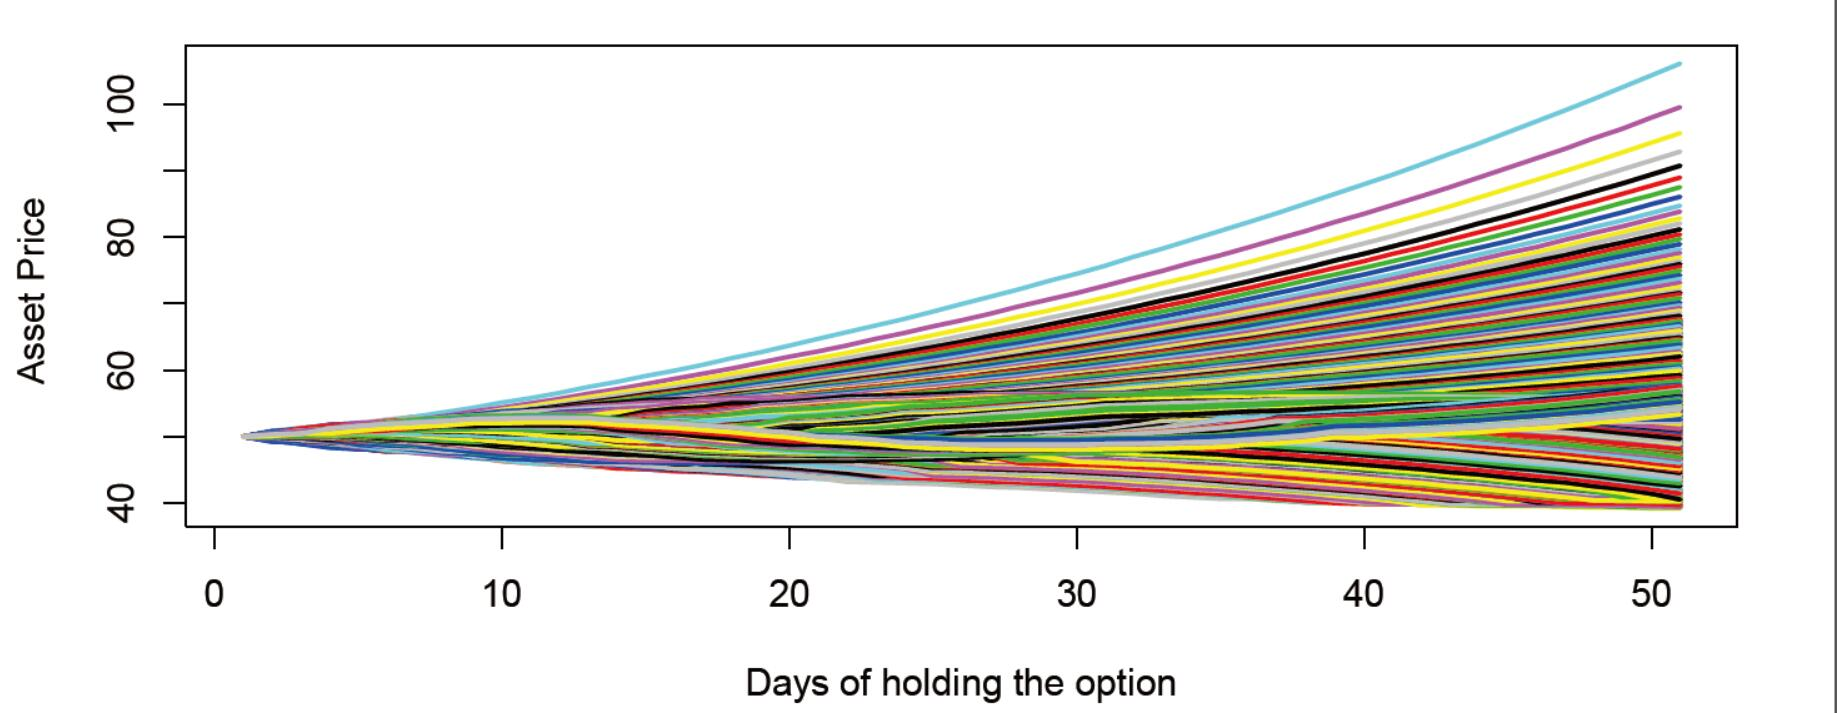
\includegraphics[width=300pt]{1.jpg}
  \caption{\href{https://github.com/SFMWISE2016/SFM10Halton_priAsiopt}{\color{blue}\textsf{SFM10Halton\_priAsiopt}}
\includegraphics[width=15pt,height=15pt]{link23.jpg}}
\end{figure}
\end{frame}
%----------------------------------------------------------------------------------------
\begin{frame}
\frametitle{APPLICATION \& RESULTS}
\begin{spacing}{1.5}
\textsf{\textbf{Step 4:}} \textsf{Averaging the asset price for each of the simulated paths and applying the appropriate formula of (2) and (3).}
\begin{eqnarray}
% \nonumber % Remove numbering (before each equation)
 \textnormal{Payoff}_{call} &=& \max(S-X,0) \\
 \textnormal{Payoff}_{put} &=& \max(X-S,0)
\end{eqnarray}
\textsf{\textbf{Step 5}}: \textsf{Averaging the payoffs for all paths  and discounting the result  to time 0.}
\end{spacing}
\end{frame}
%----------------------------------------------------------------------------------------
\begin{frame}
\frametitle{APPLICATION \& RESULTS}
\begin{spacing}{1.1}
\begin{exampleblock}{Example: How to price the Asian Call and Put options with the following parameters?}
\textsf{$X = 50$        \hspace*{20mm}   Strike at expiry}\\
\textsf{$\mu = 0.04$    \hspace*{18mm} expected return}\\
\textsf{$\sigma  = 0.1$ \hspace*{20mm}   expected vol.}\\
\textsf{$r = 0.03$      \hspace*{18mm}  Risk free rate}\\
\textsf{$dt = 1/365$    \hspace*{14mm}   time steps}\\
\textsf{$steps = 50$    \hspace*{14mm}  days to expiry}\\
\textsf{$T = dt*steps$  \hspace*{8mm}  years to expiry}\\
\textsf{$nsims = 1000$  \hspace*{8mm}   Number of simulated paths}\\

\end{exampleblock}
\begin{center}
  \href{https://github.com/SFMWISE2016/SFM10Halton_priAsiopt}{\textbf{\color{blue}\textsf{SFM10Halton\_priAsiopt}}
\includegraphics[width=15pt,height=15pt]{link23.jpg}}
\end{center}
\end{spacing}
\end{frame}
%----------------------------------------------------------------------------------------
\section{FURTHER READING}
\begin{frame}
\frametitle{FURTHER READING}
Books:
\begin{itemize}
  \item \textsf{Peter Jaeckel (2002).} \emph{Monte Carlo Methods in Finance}. \textsf{John Wiley and Sons. ISBN 0-471-49741-X.}
  \item \textsf{Bruno Dupire (1998).} \emph{Monte Carlo: Methodologies and Applications for Pricing and Risk Management. Risk.}
  \item \textsf{Don L. McLeish (2005).} \emph{Monte Carlo Simulation \& Finance.} \textsf{ISBN 0-471-67778-7.}
\end{itemize}
\end{frame}
%----------------------------------------------------------------------------------------\section{FURTHER READING}
\begin{frame}
\frametitle{FURTHER READING}
Journal:
\begin{itemize}
  \item  \emph{``Monte Carlo Simulation".} \textsf{Palisade Corporation. 2010. Retrieved 2010-09-24.}
  \item \textsf{Boyle, Phelim P.} \emph{``Options: A Monte Carlo Approach"}. \textsf{Journal of Financial Economics, Volume (Year): 4(1977), Issue (Month): 3(May). pp. 323 $-$ 338. Retrieved 2010-09-24.}
\end{itemize}
\end{frame}
%----------------------------------------------------------------------------------------
	\begin{frame}
		\frametitle{ }
		\Huge{\centerline{\textsf{\textbf{Thank you!}}}}
	\end{frame}
%----------------------------------------------------------------------------------------
	
\end{document}
